\begin{figure}[ht]
\centering
% Thesis-wide categorical color palette
% Usage: % Thesis-wide categorical color palette
% Usage: % Thesis-wide categorical color palette
% Usage: \input{figures/palette} in any figure file
%
% Muted primary colors -- print-friendly, visually distinct.
% Inspired by Cooper Union's red/blue primaries, softened for
% academic figures. Use palA-palC for data series in scatter
% plots, line charts, bar charts, etc.

\definecolor{palA}{HTML}{1F77B4}   % Tableau blue
\definecolor{palB}{HTML}{D62728}   % Tableau red
\definecolor{palC}{HTML}{2CA02C}   % Tableau green
 in any figure file
%
% Muted primary colors -- print-friendly, visually distinct.
% Inspired by Cooper Union's red/blue primaries, softened for
% academic figures. Use palA-palC for data series in scatter
% plots, line charts, bar charts, etc.

\definecolor{palA}{HTML}{1F77B4}   % Tableau blue
\definecolor{palB}{HTML}{D62728}   % Tableau red
\definecolor{palC}{HTML}{2CA02C}   % Tableau green
 in any figure file
%
% Muted primary colors -- print-friendly, visually distinct.
% Inspired by Cooper Union's red/blue primaries, softened for
% academic figures. Use palA-palC for data series in scatter
% plots, line charts, bar charts, etc.

\definecolor{palA}{HTML}{1F77B4}   % Tableau blue
\definecolor{palB}{HTML}{D62728}   % Tableau red
\definecolor{palC}{HTML}{2CA02C}   % Tableau green

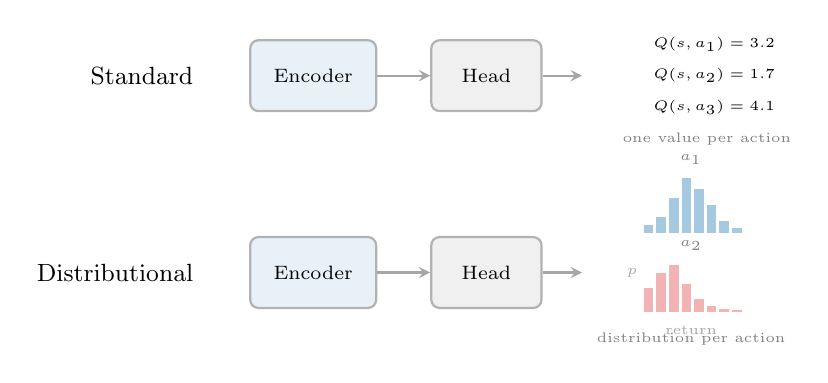
\begin{tikzpicture}[
    block/.style={draw=black!30, thick, rounded corners=3pt,
                  minimum height=0.9cm, font=\scriptsize,
                  align=center, inner sep=5pt},
    arr/.style={->, thick, >=stealth, black!35},
    lbl/.style={font=\tiny, text=black!50},
    bar/.style={thick},
]

% --- Standard DQN (top) ---
\node[font=\small, anchor=east] at (-0.6, 2.0) {Standard};

\node[block, fill=palA!10, minimum width=1.6cm]
    (enc1) at (0.8, 2.0) {Encoder};
\node[block, fill=black!6, minimum width=1.4cm]
    (head1) at (3.0, 2.0) {Head};

\draw[arr] (enc1) -- (head1);

% Scalar Q-values (one per action)
\draw[arr] (head1.east) -- ++(0.5, 0);
\foreach \i/\v in {0/3.2, 1/1.7, 2/4.1} {
    \node[font=\tiny, anchor=west] at (5.0, {2.4 - \i*0.4})
        {$Q(s, a_{\the\numexpr\i+1})=\v$};
}

\node[lbl] at (5.8, 1.2) {one value per action};

% --- Distributional (bottom) ---
\node[font=\small, anchor=east] at (-0.6, -0.5) {Distributional};

\node[block, fill=palA!10, minimum width=1.6cm]
    (enc2) at (0.8, -0.5) {Encoder};
\node[block, fill=black!6, minimum width=1.4cm]
    (head2) at (3.0, -0.5) {Head};

\draw[arr] (enc2) -- (head2);
\draw[arr] (head2.east) -- ++(0.5, 0);

% Distribution for action 1 (small bar chart)
\def\bx{5.0}
\def\by{0.0}
\foreach \i/\h in {0/0.05, 1/0.10, 2/0.22, 3/0.35, 4/0.28,
                    5/0.18, 6/0.08, 7/0.03} {
    \fill[palA!40] ({\bx + \i*0.16}, \by)
        rectangle ({\bx + \i*0.16 + 0.12}, {\by + \h*2.0});
}
\node[lbl, above] at ({\bx + 0.6}, {\by + 0.75}) {$a_1$};

% Distribution for action 2
\def\byy{-1.0}
\foreach \i/\h in {0/0.15, 1/0.25, 2/0.30, 3/0.18, 4/0.08,
                    5/0.04, 6/0.02, 7/0.01} {
    \fill[palB!35] ({\bx + \i*0.16}, \byy)
        rectangle ({\bx + \i*0.16 + 0.12}, {\byy + \h*2.0});
}
\node[lbl, above] at ({\bx + 0.6}, {\byy + 0.65}) {$a_2$};

\node[lbl] at ({\bx + 0.6}, -1.35) {distribution per action};

% Axis labels
\node[font=\tiny, text=black!35] at ({\bx - 0.15}, -0.5)
    {$p$};
\node[font=\tiny, text=black!35, anchor=north]
    at ({\bx + 0.6}, {-1.05}) {return};

\end{tikzpicture}
\caption{Distributional RL output. Standard DQN outputs one scalar
  Q-value per action; C51 outputs a probability distribution over
  possible returns for each action.}
\label{fig:distributional-output}
\end{figure}
